%//==============================--@--==============================//%
\subsection[4.1 Representação geométrica de sinais]{$\rightarrow$ Representação geométrica de sinais}
\label{subsec:geom-representation-of-signals}

A essência da representação geométrica de sinais, é decompor os $M$ sinais de energia, $\{s_i(t)\}$ numa combinação linear de $N$ funções base ortonormais, onde $N \leq M$. Isto é, dado um conjunto de sinais de energia reais, $s_1(t)$, $s_2(t)$, $\dots$, $s_M(t)$ (cada com duração $T$), podemos escrever:
$$
    s_{i}(t) = \sum_{j=1}^{N} s_{ij}\, \phi_j(t),\qquad
    \begin{cases}
        0 \leq t \leq T \\
        i = 1,2,\dots,M
    \end{cases}
$$
em que os coeficientes da expansão são dados por:
$$
    s_{ij} = \int_{0}^{T} s_i(t) \phi_j(t)\, dt,\quad
    \begin{cases}
        i = 1,2,\dots,M \\
        j = 1,2,\dots,N
    \end{cases}
$$
As funções base $\phi_1(t)$, $\phi_2(t)$, $\dots$, $\phi_N(t)$, formam um conjunto ortonormal, i.e.,
$$
    \int_{0}^{T} \phi_i(t) \phi_j(t)\, dt = \delta_{ij} =
    \begin{cases}
        1 & \text{se } i = j \\
        0 & \text{se } i \neq j
    \end{cases}
$$
onde $\delta_{ij}$ é o \textit{Kronecker delta}.

\begin{figure}[H]
    \centering
    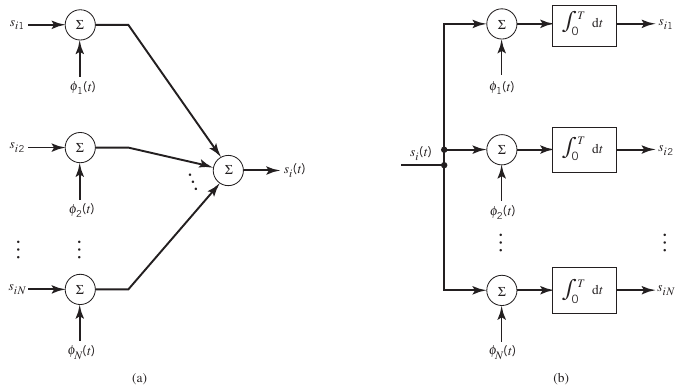
\includegraphics[width = 0.7\linewidth]{img/digital/AWGN-transmission/signals-geom-decomposition.png}
    \caption{(a) Síntese do sinal $s_i(t)$. (b) Análise para construir o vetor sinal $\{s_i\}$.}
    \label{fig:signals-geom-decomposition}
\end{figure}

\noindent Desta forma, é possível representar qualquer sinal do conjunto $\{s_i(t)\}$ sobre um vetor sinal da forma
$$
    \pmb{s}_i = 
    \begin{bmatrix}
        s_{i1}\\
        s_{i2}\\
        \vdots\\
        s_{iN}
    \end{bmatrix},\qquad i = 1,2,\dots,M
$$

\noindent O espaço euclidiano \textit{N-dimensional} onde podemos visualizar estes vetores, é denominado por \textit{signal space}/espaço de sinais.
%//==============================--@--==============================//%
\newpage
\subsubsection[4.1.1 Desigualdade de Schwarz]{$\rightarrow$ Desigualdade de Schwarz}
\label{subsubsec:shwarz}

\begin{mdframed}
Considerando um par de sinais, $s_1(t)$ e $s_2(t)$. A \textit{Desigualdade de Schwarz} afirma que
$$
    \left| \int_{-\infty}^{+\infty} s_1(t)\, s_2^*(t) \, dt \right| \leq \left( \int_{-\infty}^{+\infty} [s_1(t)]^2 \, dt \right)^{1/2}\, \left( \int_{-\infty}^{+\infty} [s_2(t)]^2 \, dt \right)^{1/2}
$$
onde o asterisco ($*$) sobrescrito denota o complexo conjugado. A igualdade apenas se verifica se, e somente se, $s_2(t) = c\, s_1(t)$, onde $c$ é uma constante arbitrária.
\end{mdframed}

%//==============================--@--==============================//%
\subsubsection[4.1.2 Processo de ortogonalização de Gram-Schmidt]{$\rightarrow$ Processo de ortogonalização de Gram-Schmidt}

\begin{theo}[\underline{Gram-Schmidt procedure}]{def:gram-schmidt}\label{def:gram-schmidt}
    Supondo um banco de $M$ sinais de energia, $s_1(t)$, $s_2(t)$, $\dots$, $s_M(t)$. Começamos por escolher um dos sinais ($s_1(t)$ sem perda de generalidade) definimos a primeira base como
    $$
        \phi_1(t) = \frac{s_1(t)}{\sqrt{E_1}}
    $$
    Definem-se em seguida as funções auxiliares
    $$
        g_i(t) = s_i(t) - \sum_{j=1}^{i-1} s_{ij}\, \phi_{j}(t),\qquad s_{ij} = \int_{0}^{T} s_i(t)\phi_j(t) \,dt 
    $$
    tal que as seguintes bases podem ser definidas como
    $$
        \phi_i(t) = \frac{g_i(t)}{\sqrt{\int_{0}^{T} [g_i(t)]^2\, dt}}
    $$
    Repare-se que para $i=1$, $g_i(t)$ reduz-se para $s_i(t)$. Verifica-se sempre que $N \leq M$ (os sinais de energia não são linearmente independentes entre si, ou, no caso limite, todos os sinais de energia são linearmente independentes).
\end{theo}

%//==============================--@--==============================//%